%%%%%%%%%%%%%%%%%%%%%%%%%%%%%%%%%%%%%%%%%%%%%%%%%%%
% CHƯƠNG 2: CƠ SỞ LÝ THUYẾT VÀ KIẾN TRÚC HỆ THỐNG
%%%%%%%%%%%%%%%%%%%%%%%%%%%%%%%%%%%%%%%%%%%%%%%%%%%
\section*{CHƯƠNG 2. CƠ SỞ LÝ THUYẾT VÀ KIẾN TRÚC HỆ THỐNG}
\addcontentsline{toc}{section}{\numberline{}CHƯƠNG 2. CƠ SỞ LÝ THUYẾT VÀ KIẾN TRÚC HỆ THỐNG}
\setcounter{section}{2}
\setcounter{subsection}{0}
\setcounter{figure}{0}
\setcounter{table}{0}

\subsection{Cơ sở y sinh học của các chỉ số đo sức khỏe}

\subsubsection{Nhịp tim (Heart Rate -- BPM) và cơ chế sinh lý}
Nhịp tim là tần số đập của tim đo bằng số nhịp co bóp tâm thất trong một phút (Beats Per Minute -- BPM). Đối với người trưởng thành khỏe mạnh bình thường ở trạng thái nghỉ ngơi, nhịp tim sinh lý dao động từ 60 đến 100 BPM. 

Cơ chế sinh lý điều hòa nhịp tim hoạt động dựa trên hệ dẫn truyền xung điện tự phát của tim:
\begin{itemize}
    \item \textbf{Nút xoang nhĩ (Sinoatrial -- SA Node):} Được ví như "máy tạo nhịp tự nhiên" nằm ở thành tâm nhĩ phải, tự phát xung điện tuần hoàn điều khiển nhịp tim.
    \item \textbf{Nút nhĩ thất (Atrioventricular -- AV Node):} Nhận xung điện từ nút xoang, trì hoãn xung điện trong khoảng vài phần trăm giây để tâm nhĩ kịp co bóp đẩy máu xuống tâm thất trước khi tâm thất co bóp.
    \item \textbf{Bó His và mạng Purkinje:} Truyền tín hiệu điện cực nhanh xuống đỉnh tim và tỏa ra xung quanh thành tâm thất, kích thích cơ tâm thất co bóp đồng loạt (chu kỳ tâm thu) để bơm máu đi khắp cơ thể.
\end{itemize}

Sự co bóp cơ tim tạo nên một làn sóng áp lực mạch đập (pulse wave) lan truyền theo dòng động mạch ngoại vi. Việc theo dõi nhịp tim giúp phát hiện sớm các bệnh lý về tim mạch. Trạng thái nhịp tim chậm (dưới 50 BPM) phản ánh cơ tim hoạt động kém hiệu quả, có nguy cơ gây thiếu máu não và ngất xỉu. Trạng thái nhịp tim nhanh (trên 120 BPM khi nghỉ ngơi) phản ánh sự quá tải của hệ tuần hoàn, dễ dẫn đến suy tim cấp hoặc rung tâm thất cực kỳ nguy hiểm.

\subsubsection{Nồng độ bão hòa oxy trong máu ($SpO_2$) và cơ chế vận chuyển oxy}
Nồng độ bão hòa oxy trong máu ngoại vi ($SpO_2$) thể hiện tỷ lệ phần trăm phân tử hemoglobin trong hồng cầu đã liên kết với oxy ($HbO_2$) trên tổng lượng hemoglobin trong dòng tuần hoàn động mạch:
\begin{equation}
    SpO_2 = \frac{C_{HbO_2}}{C_{HbO_2} + C_{Hb}} \times 100\%
\end{equation}
Trong đó $C_{HbO_2}$ là nồng độ oxyhemoglobin (hemoglobin đã bão hòa oxy) và $C_{Hb}$ là nồng độ deoxyhemoglobin (hemoglobin khử oxy). 

Oxy được hít vào phổi sẽ khuếch tán qua màng phế nang mao mạch để gắn kết phối trí với nguyên tử sắt ($Fe^{2+}$) trong nhân Heme của phân tử hemoglobin. Mỗi phân tử hemoglobin có khả năng liên kết tối đa với 4 phân tử oxy tạo thành $HbO_2$. Máu giàu oxy từ tĩnh mạch phổi được tim trái bơm đi phân phối cho toàn bộ các mô cơ quan để thực hiện quá trình hô hấp tế bào.
\begin{itemize}
    \item \textbf{Dải $SpO_2$ từ 95\% đến 100\%:} Thể hiện trạng thái trao đổi khí và tuần hoàn bình thường.
    \item \textbf{Dải $SpO_2$ từ 90\% đến 94\%:} Thể hiện trạng thái thiếu oxy nhẹ hoặc trung bình, thường gặp ở bệnh nhân hen suyễn mãn tính hoặc suy giảm chức năng phổi nhẹ.
    \item \textbf{Trạng thái $SpO_2 < 90\%$:} Tình trạng suy hô hấp cấp tính nguy kịch. Do tế bào não nhạy cảm nhất với tình trạng thiếu oxy và sẽ bắt đầu hoại tử không phục hồi sau 4-5 phút, việc sụt giảm $SpO_2$ sâu bắt buộc phải được phát hiện tức thời để bác sĩ thực hiện các can thiệp hỗ trợ thở oxy hoặc đặt nội khí quản cấp cứu.
\end{itemize}

\subsubsection{Thân nhiệt và độ ẩm da (mối liên quan sinh lý học)}
Thân nhiệt bình thường của cơ thể người đo ở các vùng trung tâm dao động ổn định trong dải $36.5^\circ\text{C}$ đến $37.2^\circ\text{C}$ nhờ cơ chế điều hòa nhiệt lượng tinh vi được điều khiển bởi vùng dưới đồi (Hypothalamus) trong não bộ. Vùng dưới đồi nhận tín hiệu từ các thụ cảm nhiệt ngoại vi trên da để điều chỉnh sự cân bằng giữa hai quá trình:
\begin{itemize}
    \item \textbf{Quá trình sinh nhiệt (Thermogenesis):} Thông qua các phản ứng chuyển hóa tế bào, sự co cơ (run rẩy) và sự phân giải mỡ.
    \item \textbf{Quá trình thải nhiệt (Thermolysis):} Thông qua cơ chế bức xạ nhiệt qua da, dẫn truyền nhiệt trực tiếp khi tiếp xúc, đối lưu không khí và bay hơi mồ hôi.
\end{itemize}
Khi cơ thể bị viêm nhiễm, các chất gây sốt nội sinh sẽ kích thích vùng dưới đồi nâng điểm đặt nhiệt (Set-point), làm thân nhiệt tăng cao ($>38.5^\circ\text{C}$). 

Nhiệt độ đo được tại bề mặt da ngoại vi (Skin Temperature) có xu hướng thấp hơn nhiệt độ trung tâm từ $0.5^\circ\text{C}$ đến $1.5^\circ\text{C}$ và chịu ảnh hưởng trực tiếp bởi sự co dãn các mạch máu dưới da. Khi kết hợp đo nhiệt độ da với độ ẩm bề mặt da (Skin Humidity), ta có thể đánh giá chính xác cơ chế thải nhiệt qua sự tiết mồ hôi. Độ ẩm da cao đột ngột đi kèm nhiệt độ da giảm mạnh thường là chỉ báo của trạng thái vã mồ hôi lạnh (diễn tiến lâm sàng nguy hiểm của sốc phản vệ hoặc nhồi máu cơ tim). Ngược lại, nhiệt độ da tăng cao nhưng độ ẩm da cực thấp thể hiện trạng thái mất nước sâu, sốt khô vô cùng nguy hiểm.

\subsection{Nguyên lý đo thể tích đồ quang học PPG}
Phương pháp quang phổ thể tích đồ (Photoplethysmography -- PPG) là kỹ thuật quang học không xâm lấn hoạt động dựa trên định luật Beer-Lambert. Định luật này mô tả sự suy giảm cường độ ánh sáng khi truyền qua một dung dịch chứa chất tan hấp thụ ánh sáng theo phương trình vi phân:
\begin{equation}
    I = I_0 \times e^{-\epsilon(\lambda) \cdot C \cdot d}
\end{equation}
Trong đó:
\begin{itemize}
    \item $I_0$ là cường độ ánh sáng phát ra ban đầu từ nguồn LED.
    \item $I$ là cường độ ánh sáng phản xạ hoặc xuyên thấu nhận được tại cảm biến quang (Photodiode).
    \item $\epsilon(\lambda)$ là hệ số hấp thụ phân tử của chất tan (hemoglobin) phụ thuộc vào bước sóng $\lambda$.
    \item $C$ là nồng độ chất tan hấp thụ (hemoglobin trong dòng máu mao mạch).
    \item $d$ là chiều dài quãng đường ánh sáng đi xuyên qua môi trường (thể tích dòng máu).
\end{itemize}

\begin{figure}[H]
    \centering
    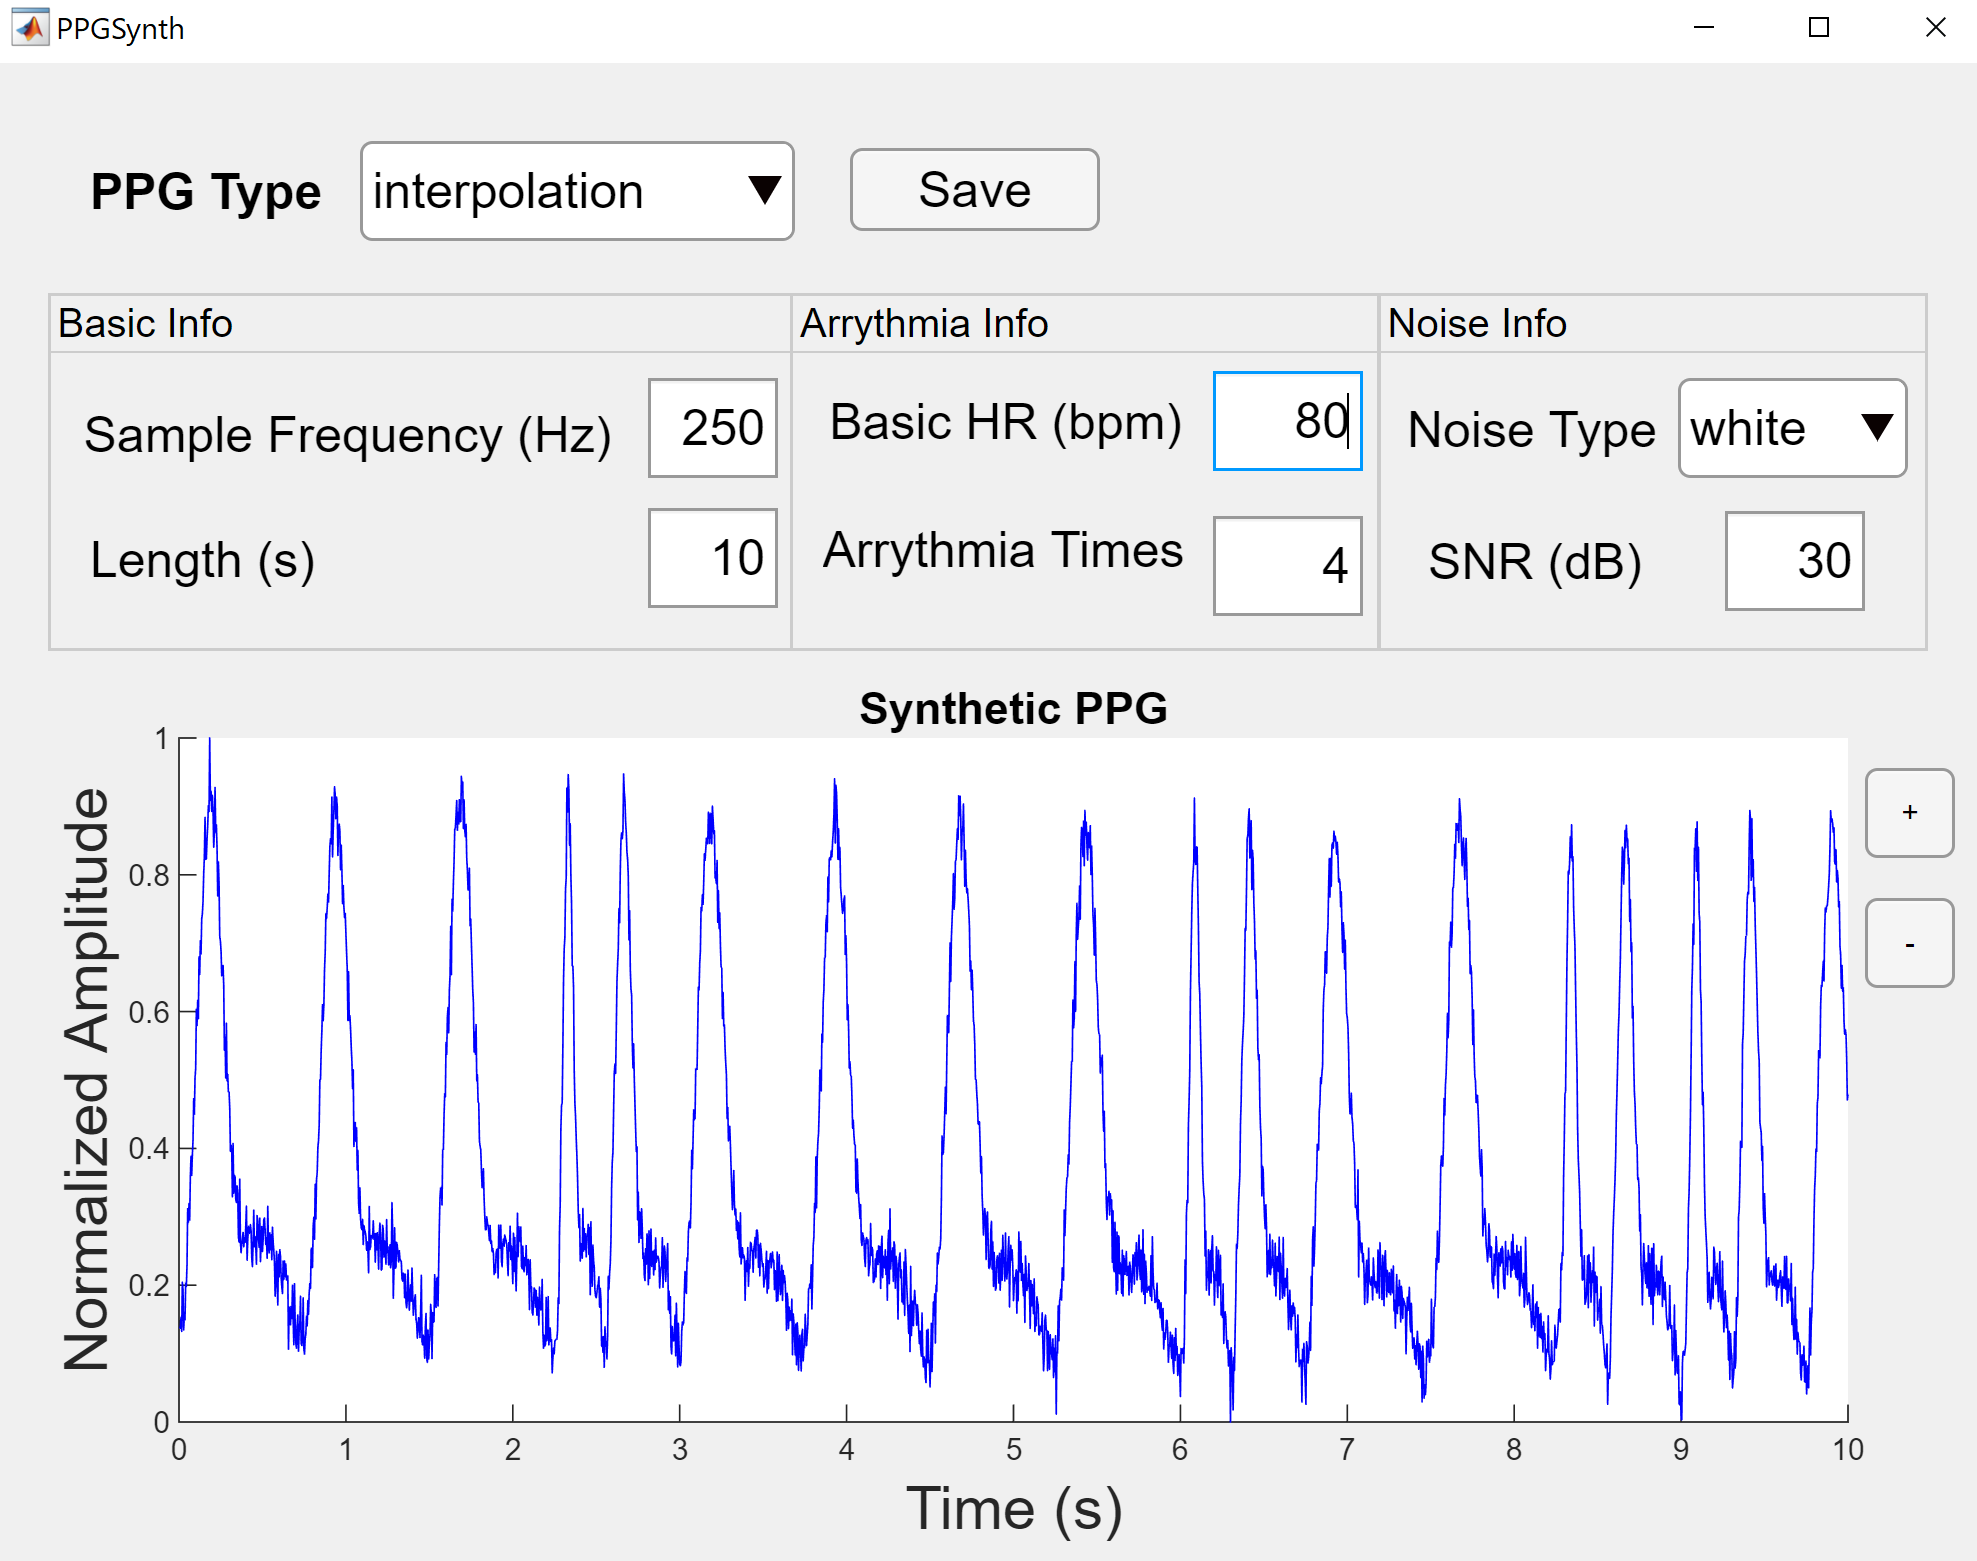
\includegraphics[width=0.8\textwidth]{images/pcb_layout.png}
    \caption[Nguyên lý thu nhận tín hiệu quang học PPG phản xạ]{\bfseries\fontsize{12pt}{0pt}\selectfont Nguyên lý thu nhận tín hiệu quang học PPG phản xạ}
    \label{fig:ppg_wavelengths_theory}
\end{figure}

Trong chu kỳ tâm thu, cơ tim co bóp mạnh đẩy một thể tích máu lớn chứa nhiều hồng cầu giàu oxy ($HbO_2$) đến hệ thống mao mạch ngoại vi ở cổ tay. Hiện tượng này làm mao mạch co dãn nở rộng ($d$ tăng), dẫn đến lượng ánh sáng bị hấp thụ bởi hồng cầu tăng lên, làm cường độ ánh sáng phản xạ $I$ nhận được tại photodiode sụt giảm xuống mức cực tiểu. 

Ngược lại, trong chu kỳ tâm trương, cơ tim dãn ra, máu rút về tim làm thể tích mao mạch sụt giảm ($d$ giảm), lượng hấp thụ giảm, cường độ ánh sáng phản xạ nhận về tăng lên cực đại. Sự dao động tuần hoàn này tạo ra sóng xung động PPG. 

Sóng PPG thu nhận được luôn bao gồm hai thành phần cơ bản:
\begin{itemize}
    \item \textbf{Thành phần xoay chiều (AC):} Đại diện cho dòng máu động mạch co bóp tuần hoàn theo nhịp tim. Thành phần này chứa thông tin tần số dao động để tính toán nhịp tim (Heart Rate).
    \item \textbf{Thành phần một chiều (DC):} Đại diện cho sự hấp thụ ánh sáng tĩnh, không thay đổi của các cấu trúc sinh học xung quanh bao gồm lớp da, cơ, mô mỡ, xương và dòng máu tĩnh mạch ổn định.
\end{itemize}

Để tính toán nồng độ bão hòa oxy $SpO_2$, ta tận dụng đặc tính hấp thụ ánh sáng hoàn toàn khác biệt của Oxyhemoglobin ($HbO_2$) và Deoxyhemoglobin ($Hb$) đối với hai bước sóng ánh sáng đặc trưng:
\begin{itemize}
    \item \textbf{Ánh sáng Đỏ (Red -- bước sóng $\approx 660\text{nm}$):} Bị hấp thụ mạnh bởi Deoxyhemoglobin ($Hb$). Do đó, máu thiếu oxy sẽ hấp thụ mạnh ánh sáng đỏ.
    \item \textbf{Ánh sáng Hồng ngoại (IR -- bước sóng $\approx 880\text{nm}$):} Bị hấp thụ mạnh bởi Oxyhemoglobin ($HbO_2$). Máu giàu oxy sẽ hấp thụ mạnh ánh sáng hồng ngoại.
\end{itemize}

Bằng cách đo đồng thời biên độ xoay chiều (AC) và thành phần tĩnh (DC) của cả hai kênh ánh sáng Đỏ và Hồng ngoại, ta tính toán tỷ số khử nhiễu $R$ (Ratio of Ratios):
\begin{equation}
    R = \frac{\text{AC}_{\text{Red}} / \text{DC}_{\text{Red}}}{\text{AC}_{\text{IR}} / \text{DC}_{\text{IR}}}
\end{equation}
Sau khi có tỷ số $R$, giá trị $SpO_2$ được nội suy tuyến tính thông qua công thức hiệu chuẩn thực nghiệm:
\begin{equation}
    SpO_2 = A - B \times R
\end{equation}
Trong đó $A$ và $B$ là các hệ số hiệu chuẩn thực nghiệm được xác định dựa trên các kiểm thử lâm sàng đối chứng. Đối với cảm biến đo ở đầu ngón tay thông thường, hệ số tiêu chuẩn thường được chọn là $A = 110.0$ và $B = 25.0$.

\subsection{Giao thức truyền thông nối tiếp I2C trong hệ thống nhúng}
Giao thức I2C (Inter-Integrated Circuit) là một chuẩn truyền thông nối tiếp đồng bộ, hai dây, hoạt động theo kiến trúc Chủ -- Tớ (Master -- Slave) do Philips Semiconductors phát triển. Giao thức này cho phép kết nối nhiều vi mạch tích hợp ngoại vi chung một bus truyền thông chỉ với 2 dây tín hiệu vật lý:
\begin{itemize}
    \item \textbf{SDA (Serial Data):} Đường truyền dữ liệu hai chiều giữa Master và các Slave.
    \item \textbf{SCL (Serial Clock):} Đường truyền xung nhịp do Master tạo ra để điều khiển tốc độ lấy mẫu dữ liệu.
\end{itemize}

Khung truyền dữ liệu I2C tiêu chuẩn diễn ra theo trình tự nghiêm ngặt sau:
\begin{enumerate}
    \item \textbf{Điều kiện Start (Start Condition):} Khi bus đang rảnh (cả hai dây SDA và SCL ở mức cao), thiết bị Master kéo đường SDA xuống mức thấp trước khi SCL chuyển sang mức thấp. Điều này đánh dấu sự bắt đầu phiên truyền tin.
    \item \textbf{Địa chỉ thiết bị (Address Frame):} Master phát ra 7 bit địa chỉ của Slave cần giao tiếp, tiếp nối bằng 1 bit hướng truyền dữ liệu R/W (Read/Write). Bit R/W = 0 nghĩa là Master muốn ghi dữ liệu vào Slave; R/W = 1 nghĩa là Master muốn đọc dữ liệu từ Slave.
    \item \textbf{Bit ACK/NACK:} Tại chu kỳ xung nhịp thứ 9 của đường SCL, Master giải phóng SDA. Thiết bị Slave có địa chỉ trùng khớp bắt buộc phải kéo đường SDA xuống mức thấp để phản hồi xác nhận (ACK -- Acknowledge). Nếu SDA giữ mức cao, Master hiểu là Slave không phản hồi (NACK -- Not Acknowledge).
    \item \textbf{Khung dữ liệu (Data Frame):} Dữ liệu được truyền theo từng byte 8-bit, bit có trọng số lớn nhất (MSB) đi trước. Mỗi byte truyền xong đều yêu cầu một bit phản hồi ACK/NACK từ phía nhận.
    \item \textbf{Điều kiện Stop (Stop Condition):} Khi kết thúc truyền dữ liệu, Master chuyển đường SDA từ mức thấp lên mức cao trong khi đường SCL đang giữ ở mức cao, đưa bus trở lại trạng thái rảnh.
\end{enumerate}

Cấu trúc vật lý của cổng I/O giao tiếp I2C sử dụng cực máng hở (Open-Drain). Do đó, các thiết bị trên bus chỉ có thể kéo dòng điện xuống mức logic 0 (GND) chứ không thể chủ động kéo điện áp lên mức logic 1 (VCC). Để duy trì mức cao khi bus rảnh, bắt buộc phải thiết kế hai điện trở kéo lên nguồn (Pull-up Resistors) cho cả hai đường SDA và SCL. 

Trị số điện trở kéo lên tối thiểu được tính toán dựa trên dòng điện chìm cực đại cho phép của bus ($I_{\text{OL}} \approx 3\text{mA}$):
\begin{equation}
    R_{\text{pullup, min}} = \frac{V_{CC} - V_{OL, max}}{I_{OL}} = \frac{3.3\text{V} - 0.4\text{V}}{3\text{mA}} \approx 966\Omega
\end{equation}
Trị số điện trở kéo lên tối đa phụ thuộc vào điện dung ký sinh tổng cộng của bus $C_b$ (gồm điện dung đường dây và chân I/O của các linh kiện) để đáp ứng thời gian tăng sườn lên (rise time $t_r$) theo tiêu chuẩn Fast Mode 400kHz ($t_r \le 300\text{ns}$):
\begin{equation}
    R_{\text{pullup, max}} = \frac{t_r}{0.8473 \cdot C_b}
\end{equation}
Với $C_b$ ước tính khoảng $100\text{pF}$, ta có $R_{\text{pullup, max}} \approx 3.54\text{k}\Omega$. Trong bo mạch thiết kế thực tế của đồ án, tôi lựa chọn trị số điện trở $R_1 = R_2 = 4.7\text{k}\Omega$ nối lên nguồn 3.3V, đảm bảo sự cân bằng tối ưu giữa việc chống nhiễu sườn xung tín hiệu và giảm thiểu tiêu hao công năng tĩnh của bus.

\subsection{Thông số kỹ thuật các linh kiện chính trong thiết kế}

\subsubsection{Vi điều khiển thế hệ mới ESP32-C3}
ESP32-C3 là dòng vi điều khiển SoC (System on Chip) giá rẻ thế hệ mới được phát triển bởi Espressif Systems. Điểm đột phá lớn nhất của ESP32-C3 là việc chuyển đổi từ kiến trúc nhân Xtensa độc quyền sang kiến trúc mã nguồn mở RISC-V 32-bit. Sự thay đổi này mang lại hiệu quả xử lý tối ưu hóa năng lượng vượt trội và khả năng tương thích phần mềm mã nguồn mở rất rộng. ESP32-C3 được thiết kế chuyên biệt để thay thế các dòng vi điều khiển 8-bit và 16-bit truyền thống trong các ứng dụng IoT gia đình thông minh và thiết bị đeo y tế nhờ tích hợp sẵn bộ phát sóng Wi-Fi và Bluetooth công nghệ năng lượng thấp (BLE) trên cùng một đế chip bán dẫn đơn diện tích cực nhỏ.

Cấu trúc phần cứng bên trong của ESP32-C3 bao gồm:
\begin{itemize}
    \item \textbf{Lõi xử lý chính:} Một nhân RISC-V 32-bit đơn nhân, cấu trúc đường ống 4 giai đoạn (4-stage pipeline), hoạt động ở tần số xung nhịp cấu hình tối đa lên tới 160 MHz. Đạt điểm số hiệu năng 4.07 CoreMark/MHz.
    \item \textbf{Hệ thống bộ nhớ nội bộ:} Tích hợp sẵn 400 KB bộ nhớ SRAM dùng cho dữ liệu và lệnh, 384 KB bộ nhớ ROM chứa mã khởi động hệ thống và các thư viện cơ bản. Hỗ trợ giao tiếp SPI Flash ngoài với dung lượng tối đa 16 MB.
    \item \textbf{Khối quản lý năng lượng (PMU):} Tích hợp bộ ổn áp nội bộ và RTC (Real-Time Clock) để điều phối 4 chế độ hoạt động tiết kiệm điện thông minh bao gồm: Active Mode, Modem-sleep Mode, Light-sleep Mode và Deep-sleep Mode.
    \item \textbf{Khối bảo mật phần cứng:} Tích hợp bộ tăng tốc mã hóa cứng hỗ trợ các chuẩn bảo mật AES-128/256, SHA-256, RSA-3072, chữ ký số (Digital Signature) và tạo số ngẫu nhiên thực (RNG), đảm bảo dữ liệu sinh học được mã hóa an toàn ngay từ phần cứng nhúng.
\end{itemize}

Mô-đun sử dụng thực tế trong đồ án là ESP32-C3-WROOM-02, được đóng gói chuẩn chân hàn bề mặt SMD với 18 chân chức năng. 
Các chân giao tiếp ngoại vi quan trọng được sử dụng bao gồm:
\begin{itemize}
    \item \textbf{GPIO8 (SDA) và GPIO9 (SCL):} Cấu hình làm bus I2C kết nối cảm biến MAX30102, HDC2022 và màn hình OLED. Chân GPIO9 đồng thời là chân BOOT khởi động cấu hình nạp.
    \item \textbf{GPIO2 (TXD) và GPIO3 (RXD):} Giao tiếp UART phục vụ việc truyền dữ liệu debug ra cổng nối tiếp khi cần thiết.
    \item \textbf{Chân EN (Chip Enable):} Chân Reset vật lý của vi điều khiển, được nối pull-up lên nguồn qua trở $10\text{k}\Omega$ và tụ lọc nhiễu $0.1\mu\text{F}$ xuống GND để chống tự reset ngẫu nhiên do nhiễu nguồn.
\end{itemize}

\begin{figure}[H]
    \centering
    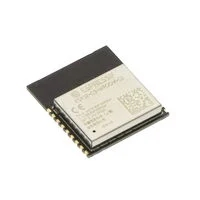
\includegraphics[width=0.35\textwidth]{images/linhkien/esp32c3.png}
    \caption[Hình ảnh thực tế module vi điều khiển ESP32-C3-WROOM-02]{\bfseries\fontsize{12pt}{0pt}\selectfont Hình ảnh thực tế module vi điều khiển ESP32-C3-WROOM-02}
    \label{fig:esp32c3_module}
\end{figure}

\subsubsection{Cảm biến nhịp tim và $SpO_2$ quang học MAX30102}
MAX30102 là cảm biến sinh trắc học quang học thế hệ mới chuyên dụng đo nhịp tim và nồng độ oxy trong máu ngoại vi ($SpO_2$) do hãng Maxim Integrated phát triển. Cảm biến này tích hợp toàn bộ các khối phát quang, thu quang và số hóa tín hiệu trong một bao gói nhựa nhỏ gọn kích thước chỉ 5.6mm x 3.3mm x 1.55mm với thấu kính thủy tinh trong suốt bảo vệ bề mặt chống bụi bẩn và tia UV môi trường.

Cấu trúc phần cứng nội bộ của MAX30102 bao gồm các khối chức năng chính:
\begin{itemize}
    \item \textbf{Khối phát quang (LED Driver):} Tích hợp 2 đèn LED có bước sóng phát quang cực kỳ chính xác: Đèn LED Đỏ phát bước sóng $\approx 660\text{nm}$ và đèn LED Hồng ngoại (IR) phát bước sóng $\approx 880\text{nm}$. Khối điều khiển LED tích hợp nguồn dòng không đổi có khả năng lập trình dòng điện phát từ 0mA đến 50mA thông qua các thanh ghi điều khiển.
    \item \textbf{Khối thu quang (Photodetector):} Tích hợp một cảm biến photodiode nhạy sáng cao, có phổ nhạy phù hợp với cả hai bước sóng ánh sáng đỏ và hồng ngoại.
    \item \textbf{Khối khử ánh sáng môi trường (Ambient Light Cancellation -- ALC):} Sử dụng mạch lọc tương tự chuyên dụng để đo cường độ ánh sáng môi trường xung quanh trước khi bật LED, sau đó trừ bớt thành phần nhiễu này ra khỏi tín hiệu thu được khi bật LED, giúp triệt tiêu hoàn toàn nhiễu từ ánh sáng mặt trời hoặc đèn huỳnh quang.
    \item \textbf{Bộ biến đổi ADC delta-sigma 18-bit:} Số hóa dòng điện tương tự từ photodiode thành giá trị số nguyên không dấu có độ phân giải cao lên tới 18-bit, tương đương dải động đạt 130dB.
\end{itemize}

MAX30102 có 8 chân kết nối vật lý dạng hàn gầm LGA:
\begin{itemize}
    \item \textbf{VDD (chân 11):} Cấp nguồn hoạt động cho mạch logic nội bộ cảm biến, điện áp từ 1.7V đến 2.0V (trong thiết kế dùng ổn áp 1.8V).
    \item \textbf{GND (chân 12):} Chân nối đất chung của cảm biến.
    \item \textbf{V\_LED+ (chân 9, 10):} Nguồn cấp trực tiếp cho các đèn LED phát quang, điện áp từ 3.1V đến 5.25V (nối lên nguồn 3.3V).
    \item \textbf{SDA (chân 2) và SCL (chân 1):} Các chân giao tiếp dữ liệu và xung nhịp của bus I2C.
    \item \textbf{INT (chân 3):} Chân ngắt cứng active-low, báo tín hiệu cho MCU khi có mẫu dữ liệu mới hoặc bộ đệm FIFO đầy.
\end{itemize}

\begin{figure}[H]
    \centering
    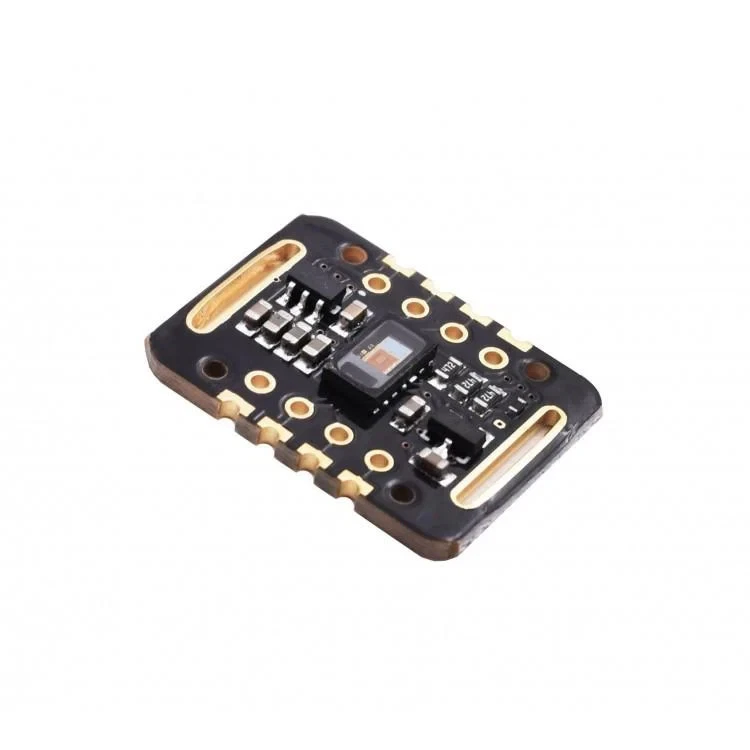
\includegraphics[width=0.35\textwidth]{images/linhkien/max30102.png}
    \caption[Hình ảnh module cảm biến nhịp tim và SpO2 MAX30102]{\bfseries\fontsize{12pt}{0pt}\selectfont Hình ảnh module cảm biến nhịp tim và SpO2 MAX30102}
    \label{fig:max30102_sensor}
\end{figure}

\subsubsection{Cảm biến nhiệt độ và độ ẩm kỹ thuật số siêu tiết kiệm điện HDC2022}
HDC2022 là cảm biến nhiệt độ và độ ẩm kỹ thuật số siêu nhỏ gọn (gói LGA 6-chân diện tích 1.5mm x 1.5mm) do Texas Instruments phát triển, tối ưu hóa đặc biệt cho các ứng dụng thiết bị đeo tay thông minh và nhà thông minh tiết kiệm năng lượng:
\begin{itemize}
    \item \textbf{Độ chính xác đo lường y tế:} Đo độ ẩm tương đối với sai số cực thấp chỉ $\pm 2\%$ trong dải từ 0\% đến 100\%. Đo nhiệt độ với sai số tối đa chỉ $\pm 0.2^\circ\text{C}$ trong dải nhiệt độ sinh lý cơ thể người hoạt động ($30^\circ\text{C}$ đến $50^\circ\text{C}$), đạt các tiêu chuẩn giám sát y tế phi lâm sàng nghiêm ngặt.
    \item \textbf{Tiêu thụ năng lượng cực thấp:} Cảm biến tiêu thụ dòng điện cực nhỏ chỉ $50\text{nA}$ ở chế độ chờ (Sleep Mode) và chỉ tiêu thụ trung bình $550\text{nA}$ khi thực hiện đo 1 lần mỗi giây ở độ phân giải 11-bit. Thiết lập này giúp kéo dài thời gian hoạt động của pin thiết bị đeo tay lên tới nhiều tháng.
    \item \textbf{Thời gian chuyển đổi ADC nhanh:} Hỗ trợ các độ phân giải cấu hình 9-bit, 11-bit hoặc 14-bit cho cả hai cảm biến, với thời gian chuyển đổi tương ứng cực kỳ nhanh (dưới 1ms).
    \item \textbf{Địa chỉ I2C cấu hình:} Địa chỉ bus I2C của HDC2022 là \texttt{0x40} (7-bit address), giao tiếp ở chế độ Fast Mode xung nhịp lên tới 400kHz.
\end{itemize}

\begin{figure}[H]
    \centering
    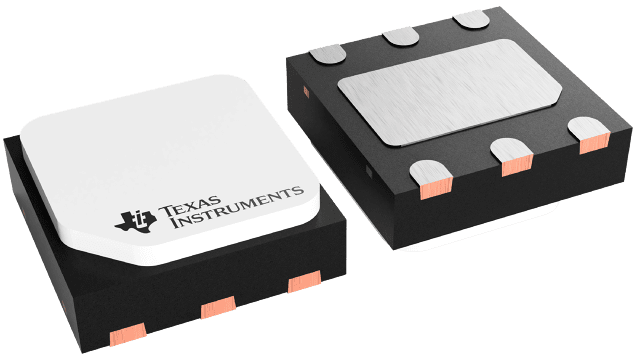
\includegraphics[width=0.35\textwidth]{images/linhkien/hdc2022.png}
    \caption[Hình ảnh module cảm biến nhiệt độ và độ ẩm HDC2022]{\bfseries\fontsize{12pt}{0pt}\selectfont Hình ảnh module cảm biến nhiệt độ và độ ẩm HDC2022}
    \label{fig:hdc2022_sensor}
\end{figure}

\subsubsection{Màn hình hiển thị OLED 0.96 inch SSD1306}
Để thực hiện hiển thị cục bộ các dữ liệu đo đạc trực quan ngay trên thiết bị đeo tay, hệ thống tích hợp màn hình OLED 0.96 inch sử dụng chip driver SSD1306. Đây là dòng màn hình hiển thị ma trận điểm đơn sắc với các đặc tính nổi bật:
\begin{itemize}
    \item \textbf{Độ phân giải hiển thị:} Đạt $128 \times 64$ điểm ảnh (pixels), cho khả năng hiển thị chữ viết, số đo sinh hiệu và đồ thị nhịp tim (sóng PPG) sắc nét và rõ ràng trên một không gian hiển thị nhỏ gọn.
    \item \textbf{Công nghệ tự phát quang (OLED):} Mỗi điểm ảnh trên màn hình tự phát sáng độc lập khi có dòng điện chạy qua mà không cần sử dụng đèn nền (backlight) như màn hình LCD. Điều này giúp màn hình đạt độ tương phản cực kỳ cao và góc nhìn rộng ($>160^\circ$), giúp người dùng dễ dàng quan sát các chỉ số sức khỏe dưới mọi điều kiện ánh sáng xung quanh.
    \item \textbf{Tiết kiệm điện năng tối đa:} Do không có đèn nền, công suất tiêu thụ của màn hình phụ thuộc trực tiếp vào số lượng điểm ảnh được bật sáng. Dòng điện tiêu thụ trung bình chỉ dao động từ $10\text{mA}$ đến $15\text{mA}$ khi hiển thị thông thường, phù hợp với các thiết bị đeo tay chạy bằng pin dung lượng nhỏ.
    \item \textbf{Chuẩn truyền thông I2C đơn giản:} Màn hình sử dụng giao tiếp I2C với địa chỉ mặc định là \texttt{0x3C}, kết nối chung bus I2C với các cảm biến MAX30102 và HDC2022 giúp tối ưu hóa số lượng chân vi điều khiển sử dụng.
\end{itemize}

\begin{figure}[H]
    \centering
    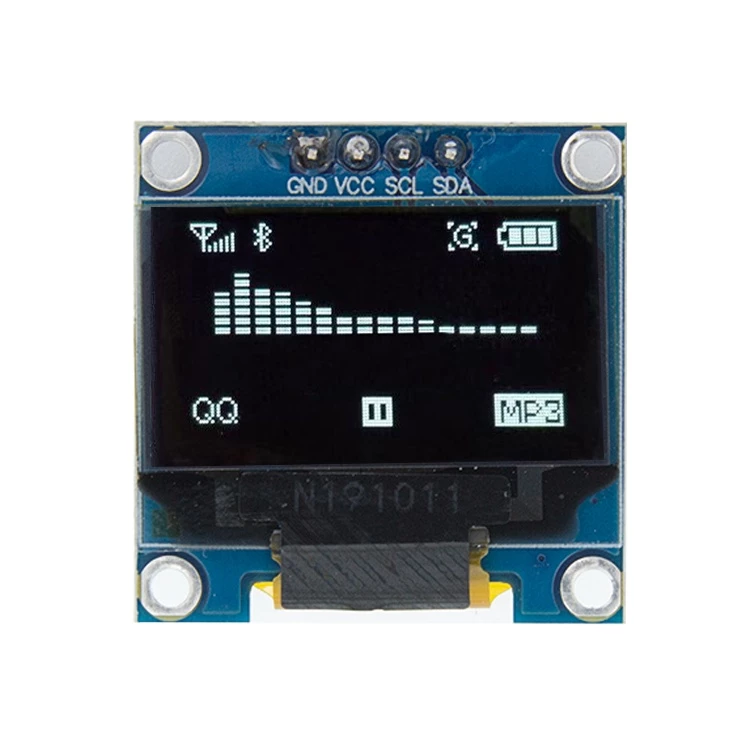
\includegraphics[width=0.35\textwidth]{images/linhkien/oled.png}
    \caption[Hình ảnh thực tế module màn hình hiển thị OLED 0.96 inch]{\bfseries\fontsize{12pt}{0pt}\selectfont Hình ảnh thực tế module màn hình hiển thị OLED 0.96 inch}
    \label{fig:oled_display}
\end{figure}

\subsubsection{Nguồn năng lượng pin Lithium-Polymer (LiPo) 3.7V}
Để đảm bảo khả năng hoạt động độc lập và di động của thiết bị đeo tay theo dõi sức khỏe, hệ thống sử dụng nguồn năng lượng từ pin Lithium-Polymer (LiPo) với các thông số kỹ thuật tối ưu:
\begin{itemize}
    \item \textbf{Dung lượng và điện áp hoạt động:} Pin có điện áp danh định $3.7\text{V}$ (điện áp khi sạc đầy đạt $4.2\text{V}$) và dung lượng $1200\text{mAh}$ (năng lượng lưu trữ đạt $4.44\text{Wh}$), cho phép thiết bị hoạt động liên tục từ 48 đến 72 giờ trong chế độ đo và truyền dữ liệu thời gian thực.
    \item \textbf{Kích thước nhỏ gọn, trọng lượng nhẹ:} Mã pin 103040 thể hiện kích thước vật lý cực kỳ mỏng nhẹ (dày 10mm, rộng 30mm, dài 40mm), phù hợp hoàn hảo với thiết kế cơ khí không gian hẹp của vỏ đồng hồ đeo tay thông minh.
    \item \textbf{Tích hợp mạch bảo vệ an toàn (PCM):} Pin được tích hợp sẵn bo mạch bảo vệ siêu nhỏ ở đầu cực để tự động ngắt nguồn khi phát hiện các sự cố quá dòng sạc, xả pin kiệt điện thế ($<2.5\text{V}$), hoặc khi xảy ra chập mạch đầu ra (short-circuit), đảm bảo an toàn tuyệt đối chống cháy nổ cho người sử dụng.
\end{itemize}

\begin{figure}[H]
    \centering
    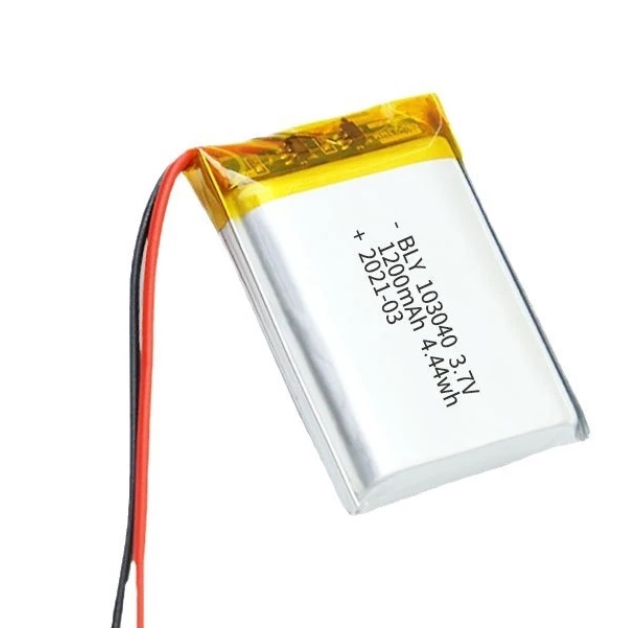
\includegraphics[width=0.35\textwidth]{images/linhkien/pin.png}
    \caption[Hình ảnh thực tế pin Lithium-Polymer 3.7V 1200mAh]{\bfseries\fontsize{12pt}{0pt}\selectfont Hình ảnh thực tế pin Lithium-Polymer 3.7V 1200mAh}
    \label{fig:lipo_battery}
\end{figure}
